\documentclass{article}
\usepackage{tikz}
\usetikzlibrary{calc,arrows}

% https://tex.stackexchange.com/questions/155401/connection-handshake-diagram-with-tikz

\begin{document}
\begin{center}
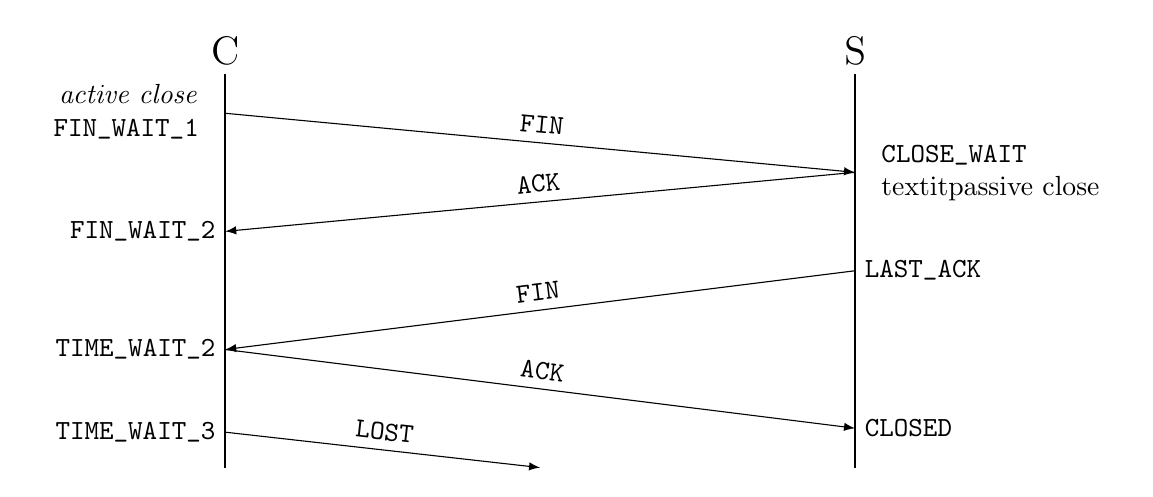
\begin{tikzpicture}[>=latex]
	% define the coordinates of client timeline
	\coordinate (A) at (0,5);
	\coordinate (B) at (0,0);
	
	% defien the coordinates of server timeline
	\coordinate (D) at (8,0);
	\coordinate (C) at (8,5);
	
	% draw client and server timeline
	\draw[thick] (A)--(B) (C)--(D);
	% label it on the top	
	\draw (A) node[above]{\Large C};
	\draw (C) node[above]{\Large S};

	\coordinate (E) at ($(A)!.1!(B)$);
	\draw (E) node[left]{
		\begin{tabular}{r}
			\textit{active close}\\
			\verb$FIN_WAIT_1$
		\end{tabular}
	};

	\coordinate (F) at ($(C)!.25!(D)$);
	\draw (F) node[right]{
		\begin{tabular}{l}
			\verb$CLOSE_WAIT$\\
			textit{passive close}
		\end{tabular}
	};
	
	
	\draw[->] (E) -- (F) node[midway,sloped,above]{\verb$FIN$};

	\coordinate (G) at ($(A)!.4!(B)$);
	\draw (G) node[left]{
		\verb$FIN_WAIT_2$
	};
	\draw[->] (F) -- (G) node[midway,sloped,above]{\verb$ACK$};

	\coordinate (H) at ($(C)!.5!(D)$);
	\draw (H) node[right]{\verb$LAST_ACK$};

	\coordinate (I) at ($(A)!.7!(B)$);
	\draw (I) node[left]{\verb$TIME_WAIT_2$};
	\draw[->] (H) -- (I) node[midway,sloped,above]{\verb$FIN$};

	\coordinate (J) at ($(C)!.9!(D)$);
	\draw (J) node[right]{\verb$CLOSED$};
	\draw[->] (I) -- (J) node[midway,sloped,above]{\verb$ACK$};
	
	\coordinate (K) at ($(I)!.7!(B)$);
	\draw (K) node[left]{\verb$TIME_WAIT_3$};
	\coordinate (Mid) at (4,0);
	\draw[->] (K) -- (Mid) node[midway,sloped, above]{\verb$LOST$};
	
\end{tikzpicture}
\end{center}
\end{document} 